%% Example data sheet
%% Feel free to modify and use this file for any purpose, under
%% either the LaTeX Project Public License or under public domain.

% Options here are passed to the article class.
% Most common options: 10pt, 11pt, 12pt
\documentclass[10pt]{datasheet}

% Input encoding and typographical rules for English language
\usepackage[utf8]{inputenc}
\usepackage[english]{babel}
\usepackage[english]{isodate}

% tikz is used to draw images in this example, but you can
% also use \includegraphics{}.
\usepackage{tikz}
\usepackage{pgfplots}
\usepackage{circuitikz}
\usetikzlibrary{calc}

% These define global texts that are used in headers and titles.
\title{Low-Tech Graphite Sensor}
\author{Mathéo HAHN et Axel LONGEPIERRE}
\date{March 2025}
\revision{Revision 1}
\companylogo{\hfill}

\begin{document}

\maketitle

\begin{tikzpicture}[remember picture, overlay, shift={(current page.south west)}]
    \node[anchor=north west] at (1.3,27) {
\includegraphics[height=2cm, keepaspectratio]{Cover/banner.png}};
\end{tikzpicture}

\section{Features}

\begin{itemize}
\item{Low power usage (3.3V-5V)}
\item{Low cost and low tech}
\item{Plug-in-play}
\item{Ergonomic and easily repairable}
\end{itemize}

\section{Applications}

\begin{itemize}
\item{Test findings of \it{Pencil Drawn Strain Gauges and Chemiresistors on Paper}\footnotemark{}}
\item{Pedagogical tool for students to design and implement their own PCB design}
\end{itemize}

\section{General Description}
This innovative sensor conceptionalized and made by students from the Applied Physics Department of INSA Toulouse is a tool inspired by the publication 
\textit{Pencil Drawn Strain Gauges and Chemiresistors on Paper}\footnotemark[\value{footnote}]. This research paper provides a simple, cost-efficient, and highly pedagogical tool for students 
to master their skills in Physics, Electronics, and Sensor Design. The sensor presented in the publication is a simple piece of paper with a layer of graphite 
on top of it, deposited by a pencil. 

Due to the graphite deposited on the piece of paper, the electrons are able to move freely from particle to particle due to quantum tunnelling. This effect is
extremely sensitive to the slightest movement of the piece of paper. We observe that compressing or stretching the graphite will change the resistivity of the 
sensor. 

\footnotetext{LIN, Cheng-Wei, ZHAO, Zhibo, KIM, Jaemyung et HUANG, Jiaxing, 2014. Pencil Drawn Strain Gauges and Chemiresistors on Paper. Scientific Reports. 22 janvier 2014. Vol.4, n°1, pp.3812. DOI 10.1038/srep03812.}

% Switch to next column
\vfill\break

\begin{figure}[h]
    \begin{circuitikz}[european]
        \node[op amp] (amp1) {};
        \node[op amp, below = 0.5cm, xscale = -1] (amp2) {};
        \draw (amp1.out) |- (amp2.-);
        \draw (amp2.-) ++(0, 0.3cm) node[circ]{} to +(2,0) node[above left]{5};
        \draw (amp2.out) to (amp1.+);
        \draw (amp1.+) ++(0, -0.3cm) node[circ]{} to +(-2,0) node[above right]{2};
        \draw (amp1.-) to +(-2,0) node[above right]{1};
        \draw (amp2.+) to +(2,0) node[above left]{4};
        \draw (amp1.out) +(0,0.5cm) node (Vdd) {$\mathrm{V_{DD}}$};
        \draw (Vdd.east) to +(1.5,0) node [above left]{6};
        \draw (amp2.out) +(0,-0.5cm) node (Vss) {$\mathrm{V_{SS}}$};
        \draw (Vss.west) to +(-1.6,0) node [above right]{3};
        \draw ($(amp1.north west) + (-0.5,0.5)$) rectangle ($(amp2.south west) + (0.5,-0.5)$);
    \end{circuitikz}
    \caption{Pinout and internal circuit}
\end{figure}

\begin{figure}[h]
    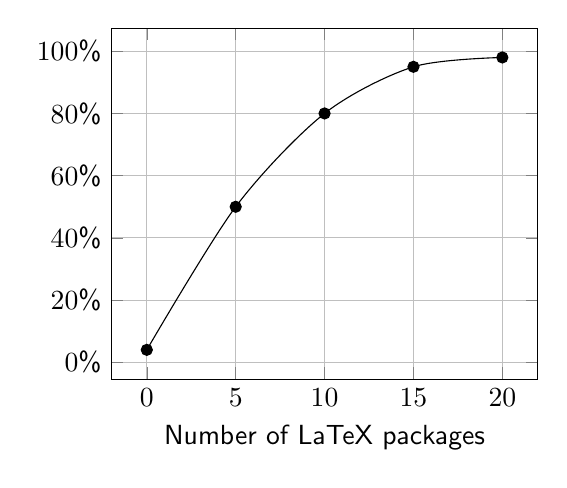
\begin{tikzpicture}
        \sffamily
        \begin{axis}[
            width=7cm,
            xlabel={Number of LaTeX packages},
            ytick distance=20,
            yticklabel={\pgfmathprintnumber{\tick}\%},
            xmajorgrids, ymajorgrids]
        \addplot[smooth,mark=*] plot coordinates {
            (0,4)
            (5,50)
            (10,80)
            (15,95)
            (20,98)
        };
        \end{axis}
    \end{tikzpicture}
    \caption{Typical data sheet production efficiency}
\end{figure}

% For wide tables, a single column layout is better. It can be switched
% page-by-page.
\onecolumn

\section{Electrical Specifications}
All specifications are in $-40\degree C \leq T_A \leq 85\degree C$ unless otherwise noted.

\begin{table}[h]
\begin{threeparttable}
\caption{Example Data Sheet Specifications}
\begin{tabularx}{\textwidth}{l | c | c c c | c | X}
    \thickhline
    \textbf{Parameter} & \textbf{Symbol} & \textbf{Min.} & \textbf{Typ.} & \textbf{Max.} &
    \textbf{Unit} & \textbf{Conditions} \\
    \hline
    Page width  & $p_w$ & 20.9 & 21.0 & 21.1 & cm & \multirow{2}{*}{Standard A4 paper} \\
    Page height & $p_h$ & 29.6 & 29.7 & 29.8 & cm &  \\
    \hline
    Insulation voltage & $E_{max}$\tnote{1} & & 1 & & kV & \\
    \thickhline
\end{tabularx}
\begin{tablenotes}
\item[1]{Based on characterization data, not tested in production.}
\end{tablenotes}
\end{threeparttable}
\end{table}

\section{Absolute Maximum Ratings}

\begin{table}[h]
\caption{Absolute Maximum Ratings of Example Data Sheet}
\begin{tabularx}{\textwidth}{l | X}
    \thickhline
    \textbf{Parameter} & \textbf{Rating} \hspace{5cm} \\
    \hline
    Daily exposure to LaTeX & 24 hours \\
    \thickhline
\end{tabularx}
\end{table}

\textbf{Note:} Stresses above those listed under Absolute Maximum Ratings can
cause permanent damage to the device. This is a stress rating only. Functional
operation of the device is not implied in any conditions above those indicated
in the Electrical Specifications section.

\end{document}


